%**************************************%
%* Generated from MathBook XML source *%
%*    on 2016-08-14T14:00:46-04:00    *%
%*                                    *%
%*   http://mathbook.pugetsound.edu   *%
%*                                    *%
%**************************************%
\documentclass[10pt,]{book}
%% Load geometry package to allow page margin adjustments
\usepackage{geometry}
\geometry{letterpaper,total={5.0in,9.0in}}
%% Custom Preamble Entries, early (use latex.preamble.early)
%% Inline math delimiters, \(, \), need to be robust
%% 2016-01-31:  latexrelease.sty  supersedes  fixltx2e.sty
%% If  latexrelease.sty  exists, bugfix is in kernel
%% If not, bugfix is in  fixltx2e.sty
%% See:  https://tug.org/TUGboat/tb36-3/tb114ltnews22.pdf
%% and read "Fewer fragile commands" in distribution's  latexchanges.pdf
\IfFileExists{latexrelease.sty}{}{\usepackage{fixltx2e}}
%% Page Layout Adjustments (latex.geometry)
%% This LaTeX file may be compiled with pdflatex, xelatex, or lualatex
%% The following provides engine-specific capabilities
%% Generally, xelatex and lualatex will do better languages other than US English
%% You can pick from the conditional if you will only ever use one engine
\usepackage{ifthen}
\usepackage{ifxetex,ifluatex}
\ifthenelse{\boolean{xetex} \or \boolean{luatex}}{%
%% begin: xelatex and lualatex-specific configuration
%% fontspec package will make Latin Modern (lmodern) the default font
\ifxetex\usepackage{xltxtra}\fi
\usepackage{fontspec}
%% realscripts is the only part of xltxtra relevant to lualatex 
\ifluatex\usepackage{realscripts}\fi
%% 
%% Extensive support for other languages
\usepackage{polyglossia}
\setdefaultlanguage{english}
%% Magyar (Hungarian)
\setotherlanguage{magyar}
%% Spanish
\setotherlanguage{spanish}
%% Vietnamese
\setotherlanguage{vietnamese}
%% end: xelatex and lualatex-specific configuration
}{%
%% begin: pdflatex-specific configuration
%% translate common Unicode to their LaTeX equivalents
%% Also, fontenc with T1 makes CM-Super the default font
%% (\input{ix-utf8enc.dfu} from the "inputenx" package is possible addition (broken?)
\usepackage[T1]{fontenc}
\usepackage[utf8]{inputenc}
%% end: pdflatex-specific configuration
}
%% Monospace font: Inconsolata (zi4)
%% Sponsored by TUG: http://levien.com/type/myfonts/inconsolata.html
%% See package documentation for excellent instructions
%% One caveat, seem to need full file name to locate OTF files
%% Loads the "upquote" package as needed, so we don't have to
%% Upright quotes might come from the  textcomp  package, which we also use
%% We employ the shapely \ell to match Google Font version
%% pdflatex: "varqu" option produces best upright quotes
%% xelatex,lualatex: add StylisticSet 1 for shapely \ell
%% xelatex,lualatex: add StylisticSet 2 for plain zero
%% xelatex,lualatex: we add StylisticSet 3 for upright quotes
%% 
\ifthenelse{\boolean{xetex} \or \boolean{luatex}}{%
%% begin: xelatex and lualatex-specific monospace font
\usepackage{zi4}
\setmonofont[BoldFont=Inconsolatazi4-Bold.otf,StylisticSet={1,3}]{Inconsolatazi4-Regular.otf}
%% end: xelatex and lualatex-specific monospace font
}{%
%% begin: pdflatex-specific monospace font
\usepackage[varqu]{zi4}
%% end: pdflatex-specific monospace font
}
%% Symbols, align environment, bracket-matrix
\usepackage{amsmath}
\usepackage{amssymb}
%% allow more columns to a matrix
%% can make this even bigger by overriding with  latex.preamble.late  processing option
\setcounter{MaxMatrixCols}{30}
%%
%% Color support, xcolor package
%% Always loaded.  Used for:
%% mdframed boxes, add/delete text, author tools
\PassOptionsToPackage{usenames,dvipsnames,svgnames,table}{xcolor}
\usepackage{xcolor}
%%
%% Semantic Macros
%% To preserve meaning in a LaTeX file
%% Only defined here if required in this document
%% Used for inline definitions of terms
\newcommand{\terminology}[1]{\textbf{#1}}
%% Subdivision Numbering, Chapters, Sections, Subsections, etc
%% Subdivision numbers may be turned off at some level ("depth")
%% A section *always* has depth 1, contrary to us counting from the document root
%% The latex default is 3.  If a larger number is present here, then
%% removing this command may make some cross-references ambiguous
%% The precursor variable $numbering-maxlevel is checked for consistency in the common XSL file
\setcounter{secnumdepth}{3}
%% Environments with amsthm package
%% Theorem-like environments in "plain" style, with or without proof
\usepackage{amsthm}
\theoremstyle{plain}
%% Numbering for Theorems, Conjectures, Examples, Figures, etc
%% Controlled by  numbering.theorems.level  processing parameter
%% Always need a theorem environment to set base numbering scheme
%% even if document has no theorems (but has other environments)
\newtheorem{theorem}{Theorem}[section]
%% Only variants actually used in document appear here
%% Style is like a theorem, and for statements without proofs
%% Numbering: all theorem-like numbered consecutively
%% i.e. Corollary 4.3 follows Theorem 4.2
%% Definition-like environments, normal text
%% Numbering is in sync with theorems, etc
\theoremstyle{definition}
\newtheorem{definition}[theorem]{Definition}
%% Example-like environments, normal text
%% Numbering is in sync with theorems, etc
\theoremstyle{definition}
\newtheorem{example}[theorem]{Example}
%% Miscellaneous environments, normal text
%% Numbering for inline exercises and lists is in sync with theorems, etc
\theoremstyle{definition}
\newtheorem{exercise}[theorem]{Exercise}
%% Localize LaTeX supplied names (possibly none)
\renewcommand*{\proofname}{Proof}
\renewcommand*{\chaptername}{Chapter}
%% Figures, Tables, Listings, Floats
%% The [H]ere option of the float package fixes floats in-place,
%% in deference to web usage, where floats are totally irrelevant
%% We re/define the figure, table and listing environments, if used
%%   1) New mbxfigure and/or mbxtable environments are defined with float package
%%   2) Standard LaTeX environments redefined to use new environments
%%   3) Standard LaTeX environments redefined to step theorem counter
%%   4) Counter for new environments is set to the theorem counter before caption
%% You can remove all this figure/table setup, to restore standard LaTeX behavior
%% HOWEVER, numbering of figures/tables AND theorems/examples/remarks, etc
%% WILL ALL de-synchronize with the numbering in the HTML version
%% You can remove the [H] argument of the \newfloat command, to allow flotation and 
%% preserve numbering, BUT the numbering may then appear "out-of-order"
\usepackage{float}
\usepackage[bf]{caption} % http://tex.stackexchange.com/questions/95631/defining-a-new-type-of-floating-environment 
\usepackage{newfloat}
% Figure environment setup so that it no longer floats
\SetupFloatingEnvironment{figure}{fileext=lof,placement={H},within=section,name=Figure}
% figures have the same number as theorems: http://tex.stackexchange.com/questions/16195/how-to-make-equations-figures-and-theorems-use-the-same-numbering-scheme 
\makeatletter
\let\c@figure\c@theorem
\makeatother
%% Raster graphics inclusion, wrapped figures in paragraphs
%% \resizebox sometimes used for images in side-by-side layout
\usepackage{graphicx}
%%
%% Program listing support, for inline code, Sage code
\usepackage{listings}
%% We define the listings font style to be the default "ttfamily"
%% To fix hyphens/dashes rendered in PDF as fancy minus signs by listing
%% http://tex.stackexchange.com/questions/33185/listings-package-changes-hyphens-to-minus-signs
\makeatletter
\lst@CCPutMacro\lst@ProcessOther {"2D}{\lst@ttfamily{-{}}{-{}}}
\@empty\z@\@empty
\makeatother
\ifthenelse{\boolean{xetex}}{}{%
%% begin: pdflatex-specific listings configuration
%% translate U+0080 - U+00F0 to their textmode LaTeX equivalents
%% Data originally from https://www.w3.org/Math/characters/unicode.xml, 2016-07-23
%% Lines marked in XSL with "$" were converted from mathmode to textmode
\lstset{extendedchars=true}
\lstset{literate={ }{{~}}{1}{¡}{{\textexclamdown }}{1}{¢}{{\textcent }}{1}{£}{{\textsterling }}{1}{¤}{{\textcurrency }}{1}{¥}{{\textyen }}{1}{¦}{{\textbrokenbar }}{1}{§}{{\textsection }}{1}{¨}{{\textasciidieresis }}{1}{©}{{\textcopyright }}{1}{ª}{{\textordfeminine }}{1}{«}{{\guillemotleft }}{1}{¬}{{\textlnot }}{1}{­}{{\-}}{1}{®}{{\textregistered }}{1}{¯}{{\textasciimacron }}{1}{°}{{\textdegree }}{1}{±}{{\textpm }}{1}{²}{{\texttwosuperior }}{1}{³}{{\textthreesuperior }}{1}{´}{{\textasciiacute }}{1}{µ}{{\textmu }}{1}{¶}{{\textparagraph }}{1}{·}{{\textperiodcentered }}{1}{¸}{{\c{}}}{1}{¹}{{\textonesuperior }}{1}{º}{{\textordmasculine }}{1}{»}{{\guillemotright }}{1}{¼}{{\textonequarter }}{1}{½}{{\textonehalf }}{1}{¾}{{\textthreequarters }}{1}{¿}{{\textquestiondown }}{1}{À}{{\`{A}}}{1}{Á}{{\'{A}}}{1}{Â}{{\^{A}}}{1}{Ã}{{\~{A}}}{1}{Ä}{{\"{A}}}{1}{Å}{{\AA }}{1}{Æ}{{\AE }}{1}{Ç}{{\c{C}}}{1}{È}{{\`{E}}}{1}{É}{{\'{E}}}{1}{Ê}{{\^{E}}}{1}{Ë}{{\"{E}}}{1}{Ì}{{\`{I}}}{1}{Í}{{\'{I}}}{1}{Î}{{\^{I}}}{1}{Ï}{{\"{I}}}{1}{Ð}{{\DH }}{1}{Ñ}{{\~{N}}}{1}{Ò}{{\`{O}}}{1}{Ó}{{\'{O}}}{1}{Ô}{{\^{O}}}{1}{Õ}{{\~{O}}}{1}{Ö}{{\"{O}}}{1}{×}{{\texttimes }}{1}{Ø}{{\O }}{1}{Ù}{{\`{U}}}{1}{Ú}{{\'{U}}}{1}{Û}{{\^{U}}}{1}{Ü}{{\"{U}}}{1}{Ý}{{\'{Y}}}{1}{Þ}{{\TH }}{1}{ß}{{\ss }}{1}{à}{{\`{a}}}{1}{á}{{\'{a}}}{1}{â}{{\^{a}}}{1}{ã}{{\~{a}}}{1}{ä}{{\"{a}}}{1}{å}{{\aa }}{1}{æ}{{\ae }}{1}{ç}{{\c{c}}}{1}{è}{{\`{e}}}{1}{é}{{\'{e}}}{1}{ê}{{\^{e}}}{1}{ë}{{\"{e}}}{1}{ì}{{\`{\i}}}{1}{í}{{\'{\i}}}{1}{î}{{\^{\i}}}{1}{ï}{{\"{\i}}}{1}{ð}{{\dh }}{1}{ñ}{{\~{n}}}{1}{ò}{{\`{o}}}{1}{ó}{{\'{o}}}{1}{ô}{{\^{o}}}{1}{õ}{{\~{o}}}{1}{ö}{{\"{o}}}{1}{÷}{{\textdiv }}{1}{ø}{{\o }}{1}{ù}{{\`{u}}}{1}{ú}{{\'{u}}}{1}{û}{{\^{u}}}{1}{ü}{{\"{u}}}{1}{ý}{{\'{y}}}{1}{þ}{{\th }}{1}{ÿ}{{\"{y}}}{1}}
%% end: pdflatex-specific listings configuration
}
%% End of generic listing adjustments
%% Sage's blue is 50%, we go way lighter (blue!05 would work)
\definecolor{sageblue}{rgb}{0.95,0.95,1}
%% Sage input, listings package: Python syntax, boxed, colored, line breaking
%% Indent from left margin, flush at right margin
\lstdefinestyle{sageinput}{language=Python,breaklines=true,breakatwhitespace=true,basicstyle=\small\ttfamily,columns=fixed,frame=single,backgroundcolor=\color{sageblue},xleftmargin=4ex}
%% Sage output, similar, but not boxed, not colored
\lstdefinestyle{sageoutput}{language=Python,breaklines=true,breakatwhitespace=true,basicstyle=\small\ttfamily,columns=fixed,xleftmargin=4ex}
%% Multiple column, column-major lists
\usepackage{multicol}
%% More flexible list management, esp. for references and exercises
%% But also for specifying labels (i.e. custom order) on nested lists
\usepackage{enumitem}
%% Lists of references in their own section, maximum depth 1
\newlist{referencelist}{description}{4}
\setlist[referencelist]{leftmargin=!,labelwidth=!,labelsep=0ex,itemsep=1.0ex,topsep=1.0ex,partopsep=0pt,parsep=0pt}
%% Lists of exercises in their own section, maximum depth 4
\newlist{exerciselist}{description}{4}
\setlist[exerciselist]{leftmargin=0pt,itemsep=1.0ex,topsep=1.0ex,partopsep=0pt,parsep=0pt}
%% Indented groups of exercises within an exercise section, maximum depth 4
\newlist{exercisegroup}{description}{4}
\setlist[exercisegroup]{leftmargin=2em,labelindent=2em,itemsep=1.0ex,topsep=1.0ex,partopsep=0pt,parsep=0pt}
%% Support for index creation
%% imakeidx package does not require extra pass (as with makeidx)
%% We set the title of the "Index" section via a keyword
%% And we provide language support for the "see" phrase
\usepackage{imakeidx}
\makeindex[title=Index, intoc=true]
\renewcommand{\seename}{see}
%% Package for tables spanning several pages
\usepackage{longtable}
%% hyperref driver does not need to be specified
\usepackage{hyperref}
%% configure hyperref's  \url  to match listings' inline verbatim
\renewcommand\UrlFont{\small\ttfamily}
%% Hyperlinking active in PDFs, all links solid and blue
\hypersetup{colorlinks=true,linkcolor=blue,citecolor=blue,filecolor=blue,urlcolor=blue}
\hypersetup{pdftitle={Applied Discrete Structures}}
%% If you manually remove hyperref, leave in this next command
\providecommand\phantomsection{}
%% If tikz has been loaded, replace ampersand with \amp macro
%% extpfeil package for certain extensible arrows,
%% as also provided by MathJax extension of the same name
%% NB: this package loads mtools, which loads calc, which redefines
%%     \setlength, so it can be removed if it seems to be in the 
%%     way and your math does not use:
%%     
%%     \xtwoheadrightarrow, \xtwoheadleftarrow, \xmapsto, \xlongequal, \xtofrom
%%     
%%     we have had to be extra careful with variable thickness
%%     lines in tables, and so also load this package late
\usepackage{extpfeil}
%% Custom Preamble Entries, late (use latex.preamble.late)
%% Begin: Author-provided macros
%% (From  docinfo/macros  element)
%% Plus three from MBX for XML characters
\newcommand{\identity}{\mathrm{id}}
\newcommand{\notdivide}{{\not{\mid}}}
\newcommand{\notsubset}{\not\subset}
\newcommand{\lcm}{\operatorname{lcm}}
\newcommand{\gf}{\operatorname{GF}}
\newcommand{\inn}{\operatorname{Inn}}
\newcommand{\aut}{\operatorname{Aut}}
\newcommand{\Hom}{\operatorname{Hom}}
\newcommand{\cis}{\operatorname{cis}}
\newcommand{\chr}{\operatorname{char}}
\newcommand{\Null}{\operatorname{Null}}
\newcommand{\lt}{ < }
\newcommand{\gt}{ > }
\newcommand{\amp}{ & }
%% End: Author-provided macros
%% Title page information for book
\title{Applied Discrete Structures}
\author{Al Doerr\\
Department of Mathematical Sciences\\
University of Massachusetts Lowell\\
\href{mailto:}{\nolinkurl{}}
\and
Ken Levasseur\\
Department of Mathematical Sciences\\
University of Massachusetts Lowell\\
\href{mailto:kenneth_levasseur@uml.edu}{\nolinkurl{kenneth_levasseur@uml.edu}}
}
\date{September, 2016}
\begin{document}
\frontmatter
%% begin: half-title
\thispagestyle{empty}
{\centering
\vspace*{0.28\textheight}
{\Huge Applied Discrete Structures}\\}
\clearpage
%% end:   half-title
%% begin: adcard
\thispagestyle{empty}
\null%
\clearpage
%% end:   adcard
%% begin: title page
%% Inspired by Peter Wilson's "titleDB" in "titlepages" CTAN package
\thispagestyle{empty}
{\centering
\vspace*{0.14\textheight}
{\Huge Applied Discrete Structures}\\[3\baselineskip]
{\Large Al Doerr}\\[0.5\baselineskip]
{\Large University of Massachusetts Lowell}\\[3\baselineskip]
{\Large Ken Levasseur}\\[0.5\baselineskip]
{\Large University of Massachusetts Lowell}\\[3\baselineskip]
{\Large September, 2016}\\}
\clearpage
%% end:   title page
%% begin: copyright-page
\thispagestyle{empty}
\vspace*{\stretch{2}}
\noindent\textcopyright\ 2016\quad{}Al Doerr, Ken Levasseur\\[0.5\baselineskip]
Applied Discrete Structures by Alan Doerr and Kenneth Levasseur is licensed under a Creative Commons Attribution-NonCommercial-ShareAlike 3.0 United States License. You are free to Share: copy and redistribute the material in any medium or format; Adapt: remix, transform, and build upon the material. You may not use the material for commercial purposes.  The licensor cannot revoke these freedoms as long as you follow the license terms.
			\par
\vspace*{\stretch{1}}
\null\clearpage
%% end:   copyright-page
%% begin: acknowledgement
\chapter*{Acknowledgements}\label{acknowledgement-1}
\addcontentsline{toc}{chapter}{Acknowledgements}
I would like to thank Rob Beezer, David Farmer and other participants on the \href{https://groups.google.com/forum/?fromgroups#!forum/mathbook-xml-support}{mathbook-xml-support group} for their guidance and work on MathBook XML.  Thanks to the Pedagogy Subcommittee of the UMass Lowell Transformational Education Committee for their financial assistance in helping getting this project started.%
%% end:   acknowledgement
%% begin: preface
\chapter*{Preface}\label{preface-1}
\addcontentsline{toc}{chapter}{Preface}
This version of \emph{Applied Discrete Structures} is being developed using \emph{Mathbook XML}, A lightweight XML application for authors of scientific articles, textbooks and monographs initiated by Rob Beezer, U. of Puget Sound.  %
\par
Sage (\href{http://sagemath.org}{sagemath.org}) is a free, open source, software system for advanced mathematics.  Sage can be used either on your own computer, a local server, or on SageMathCloud (\href{https://cloud.sagemath.com}{https://cloud.sagemath.com}). %
\par\hfill\begin{tabular}{l@{}}
Ken Levasseur\\
Lowell MA
\end{tabular}\\\par
%% end:   preface
%% begin: table of contents
\setcounter{tocdepth}{1}
\renewcommand*\contentsname{Contents}
\tableofcontents
%% end:   table of contents
\mainmatter
\typeout{************************************************}
\typeout{Chapter 1 Functions}
\typeout{************************************************}
\chapter[Functions]{Functions}\label{chapter_7}
\typeout{************************************************}
\typeout{Introduction  }
\typeout{************************************************}
In this chapter we will consider some basic concepts of the relations that are called functions. A large variety of mathematical ideas and applications can be more completely understood when expressed through the function concept.%
\typeout{************************************************}
\typeout{Section 1.1 Definition and Notation}
\typeout{************************************************}
\section[Definition and Notation]{Definition and Notation}\label{s-function-def-notation}
\typeout{************************************************}
\typeout{Subsection 1.1.1 Fundamentals}
\typeout{************************************************}
\subsection[Fundamentals]{Fundamentals}\label{ss-fundamentals-functions}
\begin{definition}[ Function]\label{def-function}
\index{Function}\label{notation-1}
A function from a set \(A\) into a set \(B\) is a relation from \(A\) into \(B\) such that each element of \(A\) is related to exactly one element of the set \(B\). The set \(A\) is called \terminology{domain} of the function and the set \(B\) is called the \terminology{codomain}.%
\end{definition}
The reader should note that a function \(f\) is a relation from \(A\) into \(B\) with two important restrictions:%
\par
\leavevmode%
\begin{itemize}[label=\textbullet]
\item{} Each element in the set \(A\), the domain of \(f\), must be related to some element of \(B\), the codomain.%
\item{}The phrase ``is related to exactly one element of the set B'' means that if \((a, b)\in f\) and \((a, c)\in f\), then \(b = c\).%
\end{itemize}
%
\begin{example}[A function as a list of ordered pairs]\label{ex-function-1}
Let \(A = \{-2, -1,0, 1, 2\}\) and \(B = \{0, 1, 2, 3, 4\}\), and if \(s = \{(-2, 4), (-1, 1), (0, 0), (1, 1), (2, 4)\}\), then \(s\) is a function from \(A\) into \(B\).%
\end{example}
\begin{example}[A function as a set of ordered pairs in set-builder notation]\label{ex-function-2}
Let \(\mathbb{R}\) be the real numbers. Then \(L = \{(x, 3x) \mid x \in \mathbb{R}\}\) is a function from \(\mathbb{R}\) into \(\mathbb{R}\),
or, more simply, \(L\) is a function on \(\mathbb{R}\).%
\end{example}
\par
It is customary to use a different system of notation for functions than the one we used for relations. If \(f\) is a function from the set  \(A\) into the set \(B\), we will write \(f:A \rightarrow B\).%
\par
The reader is probably more familiar with the notation for describing functions that is used in basic algebra or calculus courses. For example, \(y =\frac{1}{x}\) or \(f(x) =\frac{1}{x}\) both define the function \(\left\{\left.\left(x,\frac{1}{x}\right)\right| x\in \mathbb{R}, x\neq
0\right\}\). Here the domain was assumed to be those elements of \(\mathbb{R}\) whose substitutions for \(x\) make sense, the nonzero real numbers,
and the codomain was assumed to be \(\mathbb{R}\). In most cases, we will make a point of listing the domain and codomain in addition to describing what the function does in order to define a function. %
\par
The terms \terminology{mapping}, \terminology{map}, and \terminology{transformation} are also used for functions.%
\par
One way to imagine a function and what it does is to think of it as a machine. The machine could be mechanical, electronic, hydraulic, or abstract. Imagine that the machine only accepts certain objects as raw materials or input. The possible raw materials make up the domain. Given some input, the machine produces a finished product that depends on the input. The possible finished products that we imagine could come out of this process make up the codomain.%
\begin{example}[A definition based on images]\label{ex-non-pair-description}
We can define a function based on specifying the codomain element to which each domain element is related.   For example, f: \(\mathbb{R} \rightarrow \mathbb{R}\) defined by \(f(x) = x^2\) is an alternate description of \(f= \left\{\left.\left(x,
x ^2\right)\right|x \in  \mathbb{R}\right\}\).%
\end{example}
\begin{definition}[Image of an element under a function]\label{def-image-of-an-element}
\index{Image of an Element.}\label{notation-2}
Let \(f:A \rightarrow  B\), (read ``Let \(f\) be a function from the set \(A\) into
the set \(B\).'') If \(a \in  A\), then \(f(a)\) is used to denote that element of \(B\) to which \(a\) is related.
\(f(a)\) is called the \terminology{image} of \(a\), or, more precisely, the image of \(a\) under \( f\). We write \(f(a) = b\) to indicate that the image of \(a\) is \(b\).%
\end{definition}
\par
In \hyperref[ex-non-pair-description]{Example~\ref{ex-non-pair-description}}, the image of 2 under \(f\) is 4; that is, \(f(2) = 4\). In \hyperref[ex-function-1]{Example~\ref{ex-function-1}}, the image of -1 under \(s\) is 1; that is,
\(s(-1) = 1\).%
\begin{definition}[Range of a Function]\label{def-range-of-function}
\index{Range of a Function.}\label{notation-3}
 The range of a function is the set of images of its domain. If \(f:X \rightarrow Y\), then the range of f is denoted \(f(X)\), and  
\begin{equation*}f(X) = \{f(a) \mid a \in X\} = \{b \in Y \mid  \exists a \in X\textrm{ such that } f(a) = b\}\end{equation*}%
\end{definition}
\par
Note that the range of a function is a subset of its codomain. \(f(X)\) is also read as ``the image of the set \(X\) under the function \(f\)`` or simply ''the image of \(f\).''%
\par
In \hyperref[ex-function-1]{Example~\ref{ex-function-1}}, \(s(A)= \{0, 1, 4\}\). Notice that 2 and 3 are not images of any element of \(A\). In addition, note that both 1 and 4 are related to more than one element of the domain \(s(1) = s(-1) = 1\) and \(s(2) = s(-2) = 4\). This does not violates the definition of a function. Go back and read the definition if this isn't clear to you.%
\par
In \hyperref[ex-function-2]{Example~\ref{ex-function-2}}, the range of \(L\) is equal to its codomain, \(\mathbb{R}\). If \(b\) is any real number, we can demonstrate that it
belongs to L(\(\mathbb{R}\)) by finding a real number \(x\) for which \(L(x) = b\). By the definition of \(L\), \(L(x) = 3x\), which leads
us to the equation \(3x = b\). This equation always has a solution, \(\frac{b}{3}\); thus \(L(\mathbb{R}) = \mathbb{R}\).%
\par
The formula that we used to describe image of a real number under \(L\), \(L(x) = 3x\), is preferred over the set notation for \(L\)
due to its brevity. Any time a function can be described with a rule or formula, we will use this form of description. In Example 7.1.1, the image
of each element of \(A\) is its square. To describe that fact, we write \(s(a) = a^2\) (\(a \in  A\)), or \(S:A \rightarrow  B\) defined by
\(S(a) = a^2\).%
\par
There are many ways that a function can be described. Many functions, such as the complexity of the function dictate its representation.%
\begin{example}[Data as a function]\label{ex-data-function}
Suppose a survey of 1,000 persons is done asking how many hours of television each watches per day. Consider the function \(W:
\{0,1,\ldots , 24\} \rightarrow  \{0,1,2,\ldots ,1000\}\) defined by 
 \[W(t) = \textrm{the number of persons who gave a response of } t \textrm{ hours}\] 

This function will probably have no formula such as the ones for s and L above. Besides listing the data in a table, a bar graph might be a good
way to represent \(W\).%
\end{example}
\begin{example}[Conditional definiton of a function]\label{ex-conditional-function}
 Consider the function \(m:\mathbb{P} \rightarrow  \mathbb{Q}\) defined by the set

\begin{equation*}m = \{(1, 1), (2, 1/2), (3, 9), (4, 1/4), (5, 25), . . . \} \end{equation*}

No simple single formula could describe \(m\), but if we assume that the pattern given continues, we can write

 \begin{equation*}m(x) =\left\{
\begin{array}{cc}
 x^2 &  \textrm{if } x \textrm{ is odd} \\
 1/x & \textrm{if } x \textrm{ is even} \\
\end{array}
\right.\end{equation*}
%
\end{example}
\typeout{************************************************}
\typeout{Subsection 1.1.2 Functions of Two Variables}
\typeout{************************************************}
\subsection[Functions of Two Variables]{Functions of Two Variables}\label{ss-two-variables}
\index{Functions!Of two Variables}If the domain of a function is the Cartesian product of two sets, then our notation and terminology is changed slightly. For example, consider the
function \(C:\mathbb{N} \times \mathbb{N}\rightarrow \mathbb{N}\) defined by \(C\left(\left(n_1,n_2\right)\right)=n_1^2+n_2^2- n_1n_2+10\).  For
this function, we would drop one set of parentheses and write \(C(4, 2) = 22\), not \(C((4, 2)) = 22\). We call \(C\) a function of two variables.
From one point of view, this function is no different from any others that we have seen. The elements of the domain happen to be slightly more complicated.
On the other hand, we can look at the individual components of the ordered pairs as being separate. If we interpret \(C\) as giving us the cost of
producing quantities of two products, we can imagine varying \(n_1\) while \(n_2\) is fixed, or vice versa.%
\typeout{************************************************}
\typeout{Subsection 1.1.3 Sage Note}
\typeout{************************************************}
\subsection[Sage Note]{Sage Note}\label{ss-sage-note-functions}
\index{Sage Note!Functions}There are several ways to define a function in Sage. The simplest way to implement \(f\) is as follows.%
\begin{lstlisting}[style=sageinput]
f(x)=x^2
f
\end{lstlisting}
\begin{lstlisting}[style=sageoutput]
x |--> x^2
\end{lstlisting}
\begin{lstlisting}[style=sageinput]
[f(4),f(1.2)]
\end{lstlisting}
\begin{lstlisting}[style=sageoutput]
[16,1.44000000000000]
\end{lstlisting}
\par
Sage is built upon the programming language Python, which is a \emph{strongly typed language} and so you can't evaluate expressions such as \(f(``Hello'')\). However a function like f above will accept any type of number, so a bit more work is needed to restrict the inputs of f to the integers.%
\par
A second way to define a function in Sage is based on Python syntax.%
\begin{lstlisting}[style=sageinput]
def fa(x):
	return x^2
[fa(2),fa(1.2)]
\end{lstlisting}
\begin{lstlisting}[style=sageoutput]
[16,1.44000000000000]
\end{lstlisting}
\typeout{************************************************}
\typeout{Subsection 1.1.4 Non-Functions}
\typeout{************************************************}
\subsection[Non-Functions]{Non-Functions}\label{ss-non-functions}
We close this section with two examples of relations that are not functions.%
\begin{example}[A non-function]\label{ex-nonfunction1}
 Let \(A = B = \{1, 2, 3\}\) and let \(f= \{(1, 2), (2, 3)\}\). Here \(f\) is not a function since \(f\) does not
act on, or ``use,'' all elements of \(A\).%
\end{example}
\begin{example}[Another non-function]\label{ex-nonfunction2}
 Let \(A = B = \{1,2, 3\}\) and let \(g = \{(1, 2), (2, 3), (2, 1),(3, 2)\}\). We note that \(g\) acts on all of \(A\).  However, \(g\) is still not a function since \((2, 3) \in  g\) and \((2, 1) \in  g\) and the condition on each domain being related
to exactly one element of the codomain is violated.%
\end{example}
\typeout{************************************************}
\typeout{Exercises 1.1.5 Exercises for Section 7.1 }
\typeout{************************************************}
\subsection[Exercises for Section 7.1 ]{Exercises for Section 7.1 }\label{exercises-7-1}
\hypertarget{exercisegroup-1}{}\typeout{************************************************}
\typeout{Introduction  }
\typeout{************************************************}
A Exercises%
\begin{exercisegroup}
\item[1.]\hypertarget{exercise-1}{} Let \(A = \{1, 2, 3, 4\}\) and \(B = \{a,b, c, d)\). Determine which of the following are functions. Explain.%
\par
\leavevmode%
\begin{enumerate}[label=\alph*]
\item\hypertarget{li-3}{} \(f \subseteq  A \times  B\), where \(f = \{(1, a), (2, b), (3, c), (4, d)\}\).%
\item\hypertarget{li-4}{} \(g\subseteq A\times B\), where \(g = \{(1, a), (2, a), (3,b), (4,d)\}\).%
\item\hypertarget{li-5}{} \(h \subseteq A \times  B\), where \(A = \{(1, a), (2, b), (3, c)\}\).%
\item\hypertarget{li-6}{} \(k \subseteq A\times  B\), where \(k = \{(1, a), (2, b), (2, c), (3, a), (4, a)\}\).%
\item\hypertarget{li-7}{} \(L\subseteq A\times A\), where \(L = \{(1, 1), (2, 1), (3, 1), (4, 1)\}\).%
\end{enumerate}
%
\par\smallskip
\par\smallskip
\noindent\textbf{Answer.}\hypertarget{answer-1}{}\quad
\leavevmode%
\begin{multicols}{3}
\begin{enumerate}[label=\alph*]
\item\hypertarget{li-8}{} Yes %
\item\hypertarget{li-9}{} Yes %
\item\hypertarget{li-10}{} No %
\item\hypertarget{li-11}{}No%
\item\hypertarget{li-12}{}Yes%
\end{enumerate}
\end{multicols}
%
\item[2.]\hypertarget{exercise-characteristic-function}{} Let \(A\) be a set and let \(S\) be any subset of \(A\). Let \(\chi _S: A\to \{0,1\}\) be defined by



\begin{equation*}\chi _S(x)= \left\{
\begin{array}{cc}
 1 & \textrm{if } x\in S \\
 0 & \textrm{if } x\notin S \\
\end{array}
\right.
\end{equation*}
%
\par
The function \(\chi _S\), is called the \terminology{characteristic function}\index{Characteristic function} of \(S\)%
\par
\leavevmode%
\begin{enumerate}[label=(\alph*)]
\item\hypertarget{li-13}{} If \(A = \{a, b, c\}\) and \(S = \{a, b\}\), list the element of \(\chi _S\) .%
\item\hypertarget{li-14}{} If \(A = \{a, b, c, d, e\}\) and \(S = \{a, c, e\}\), , list the element of \(\chi _S\).%
\item\hypertarget{li-15}{} If \(A = \{a, b, c\}\), what are \(\chi _{\emptyset }\) and \(\chi _A\).%
\end{enumerate}
%
\par\smallskip
\item[3.]\hypertarget{exercise-3}{} Find the ranges of each of the relations that are functions in Exercise 1.%
\par\smallskip
\par\smallskip
\noindent\textbf{Answer.}\hypertarget{answer-2}{}\quad
\leavevmode%
\begin{enumerate}[label=\alph*]
\item\hypertarget{li-16}{} Range of \(f=f(A)=\{a,b,c,d\}=B\)%
\item\hypertarget{li-17}{} Range of \(g=g(A)=\{a,b,d\}\)%
\item\hypertarget{li-18}{} Range of \(L=L(A)=\{1\}\)%
\end{enumerate}
%
\item[4.]\hypertarget{exercise-4}{} Find the ranges of the following functions on \(\mathbb{Z}\):%
\par
\leavevmode%
\begin{enumerate}[label=\alph*]
\item\hypertarget{li-19}{} \(g = \{(x, 4x +1)|x \in  \mathbb{Z}\}\)%
\item\hypertarget{li-20}{} \(h(x) = \text{least} \text{integer} \text{that} \text{is} \text{greater} \text{than} \text{or} \text{equal} \text{to} \sqrt{|x|}\).%
\item\hypertarget{li-21}{} \(P(x) = x + 10\).%
\end{enumerate}
%
\par\smallskip
\item[5.]\hypertarget{exercise-5}{} Let \(f:\mathbb{P}\to \mathbb{P}\), where\(f(a)\) is the largest power of two that evenly divides \(a\); for example, \(f(12)=4,f(9)=1,\text{and}
f(8)=8\). Describe the equivalence classes of the kernel of \(f\).%
\par\smallskip
\item[6.]\hypertarget{exercise-6}{} Let \(U\) be a set with subsets \(A\) and \(B\).%
\par
\leavevmode%
\begin{enumerate}[label=\alph*]
\item\hypertarget{li-22}{} Show that \(g:U\to \{0,1\}\) defined by \(g(a)=\min \left(C_A(a),C_B(a)\right)\) is the characteristic function of \(A\cap B\).%
\item\hypertarget{li-23}{} What characteristic function is \(h:U\to \{0,1\}\) defined by \(h(a)=\max \left(C_A(a),C_B(a)\right)\)?%
\item\hypertarget{li-24}{} How are the characteristic functions of \(A\) and \(A^c\) related?%
\end{enumerate}
%
\par\smallskip
\end{exercisegroup}
\par\smallskip\noindent
\hypertarget{exercisegroup-2}{}\typeout{************************************************}
\typeout{Introduction  }
\typeout{************************************************}
B Exercises%
\begin{exercisegroup}
\item[7.]\hypertarget{exercise-7}{}If \(\lvert A \rvert\) and \(\lvert B \rvert\) are both finite, how many different functions are there from \(A\) into \(B\)?%
\par\smallskip
\par\smallskip
\noindent\textbf{Answer.}\hypertarget{answer-3}{}\quad
 For each of the \(\lvert A \rvert \) elements of \(A\), there are \(\lvert B \rvert\) possible images, so there are\(\lvert B \rvert\cdot \lvert B \rvert\cdot \ldots \cdot \lvert B \rvert=\left\lvert B \rvert^{\lvert A \rvert}\right.\) functions from \(A\) into \(B\).%
\item[8.]\hypertarget{exercise-8}{} Let \(f\) be a function with domain \(A\) and codomain \(B\). Consider the relation \(K \subseteq  A \times  A\) defined
on the domain of \(f\) by \((x, y) \in  K\) if and only if \(f(x) = f(y)\). The relation \(K\) is called \textit{ the kernel of f}.%
\par
\leavevmode%
\begin{enumerate}[label=\alph*]
\item\hypertarget{li-25}{} Prove that \(K\) is an equivalence relation.%
\item\hypertarget{li-26}{} For the specific case of \(A = \mathbb{Z}\), where \(\mathbb{Z}\) is the set of integers, let \(f: \mathbb{Z} \rightarrow  \mathbb{Z}\) be defined by \(f(x) = x^2\). Describe the equivalence classes of the kernel for this specific function.%
\end{enumerate}
%
\par\smallskip
\end{exercisegroup}
\par\smallskip\noindent
\typeout{************************************************}
\typeout{Section 1.2 Properties of Functions }
\typeout{************************************************}
\section[Properties of Functions ]{Properties of Functions }\label{s-properties-of-functions}
\index{Properties of Functions}Consider the following functions:%
\par
Let \(A = \{1, 2, 3, 4\}\) and \(B = \{a, b, c, d\}\), and defined \(f:A \rightarrow  B\) by 
\begin{equation*}f(1) = a, f(2) = b, f(3) = c \textrm{ and } f(4) = d\end{equation*}
%
\par
Let \(A = \{1, 2, 3, 4\}\) and \(B = \{a, b, c, d\}\), and defined \(g:A \rightarrow  B\) by 
\begin{equation*}g(1) = a , g(2) = b, g(3) = a \textrm{ and } g(4) = b.\end{equation*}
%
\par
The first function, \(f\), gives us more information about the set \(B\) than the second function, \(g\). Since \(A\) clearly has four elements,/tells us that the set \(B\) contains at least four elements since each element of the set \(A\) is mapped onto one and only one element of the set \(B\), The properties that f has, and g does not have, are the most basic properties that we look for in a function. The following definitions summarize the basic vocabulary for function properties.%
\begin{definition}[Injective Function, Injection]\label{def-injective-function}
\index{Function!Injective}\index{Function!One-to-one}\index{Injection}A function \(f: A \rightarrow B\) is injective if \begin{equation*} a, b\in  A, a\neq b \Rightarrow  f(a) \neq  f(b)\end{equation*}  A injective function is called a injection, or a one-to-one function%
\end{definition}
\par
Notice that the condition for a injective function is equivalent to
  \[a, b\in  A, f(a) = f(b) \Rightarrow  a = b\] 
%
\begin{definition}[Surjective Function, Surjection]\label{def-surjective-function}
\index{Function!Surjective}\index{Function!Onto}\index{Surjection}A function \(f: A \rightarrow B\) is surjective if its range, \(f(A)\), is equal to its codomian B.  A surjective function is called a surjection, or an onto function%
\end{definition}
\par
Notice that the condition for a surjective function is equivalent to 
\begin{equation*}\textrm{For all } b \in  B\textrm{, there exists } a\in A \textrm{ such that } f(a)=b.\end{equation*}%
\begin{definition}[Bijective Function, Bijection.]\label{def-bijective-function}
\index{Function!Bijective}\index{Bijection} A function \(f: A \rightarrow B\) is bijective if it is both injective and surjective. Bijective functions are also called one-to-one, onto functions.%
\end{definition}
\par
The function \(f\) that we opened this section with is bijective. The function \(g\) is neither injective nor
surjective.%
\begin{example}[Injective but not surjective function]\label{ex-injective-notsurjective}
Let \(A = \{1, 2, 3\}\) and \(B = \{a, b, c, d\}\), and define \(f:A \rightarrow  B\) by \(f(1) = b\), \(f(2) = c\), and \(f(3)
= a\). Then \( f \) is injective but not surjective.%
\end{example}
\begin{example}[Characteristic Functions]\label{ex-characteristic-properties}
The characteristic function, \(\chi _S\) in \hyperlink{exercise-characteristic-function}{Exercise~1.1.5.2}  is surjective if \(S\) is a proper subset of \(A\), but never injective if \(\lvert A \rvert > 2\).%
\end{example}
\begin{example}[Seating Students]\label{ex-classroom}
Let \(A\) be the set of students who are sitting in a classroom,  let \(B\) be the set of seats in the classroom, and let \(s\) be the function which maps each student into the chair he or she is sitting in. When is \(s\) one to one? When is it onto? Under normal circumstances, \(s\)  would always be injective since no two different students would be in the same seat.  In order for \(s\) to be surjective, we need all seats to be used, so \(s\)  is a surjection if the classroom is filled to capacity.%
\end{example}
\par
Functions can also be used for counting the elements in large finite sets or in infinite sets. Let's say we wished to count the occupants in an auditorium containing 1,500 seats. If each seat is occupied, the answer is obvious, 1,500 people. What we have done is to set up a one-to-one correspondence, or bijection, from seats to people. We formalize in a definition.%
\begin{definition}[Cardinality.]\label{def-cardinality}
\index{Cardinality.}\label{notation-4}
Two sets are said to have the same cardinality if there exists a bijection between them. If a set has the same cardinality as the set \(\{1,2,3,\ldots , n\}\), then we say its cardinality is \(n\).  %
\end{definition}
\par
The function \(f\) that opened this section serves to show that the two sets \(A=\{1, 2, 3, 4\}\) and \(B=\{a, b, c, d\}\) have the same cardinality. Notice in applying the definition of cardinality, we don't actually appear to count either set, we just match up the elements. However, matching the letters in \(B\) with the numbers 1, 2, 3, and 4 is precisely how we count the letters.%
\begin{definition}[ Countable Set.]\label{def-countable-set.}
\index{Countable Set}If a set is finite or has the same cardinality as the set of positive integers, it is called a countable set.%
\end{definition}
\begin{example}[Counting the Alphabet]\label{ex-the-alphabet}
 The alphabet \(\{A, B, C, . . . , Z\}\) has cardinality 26 through the following bijection into the set \(\{1,2,3,\ldots ,26\}\)
\begin{equation*}
\begin{array}{ccccc}
 A & B & C & \cdots  & Z \\
 \downarrow  & \downarrow  & \downarrow  & \cdots  & \downarrow  \\
 1 & 2 & 3 & \cdots  & 26 \\
\end{array}
\end{equation*}%
\end{example}
\par
Recall that \(2\mathbb{P}= \{b\in \mathbb{P} \mid b= 2k \textrm{ for some } k \in \mathbb{P} \}\)%
\begin{example}[As many evens as all positive integers]\label{ex-evens-eq-all}
Paradoxically, the set \(2\mathbb{P}\) of even positive integers has the same cardinality as the set \(\mathbb{P}\) of positive integers. To prove this, we must find a bijection from \(\mathbb{P}\) to \(2\mathbb{P}\).  Such a function isn't unique, but this one is the simplest: \(f:\mathbb{P} \rightarrow  2\mathbb{P}\) where \(f(m) = 2m\).  Two statements must be proven to justify our claim that \(f\) is a bijection:%
\par
\leavevmode%
\begin{itemize}[label=\textbullet]
\item{} \(f\) is one-to-one.%
\par
Proof: Let \(a, b \in  \mathbb{P}\) and assume that \(f(a) = f(b)\). We must prove that \(a = b\). 
\begin{equation*} f(a) = f(b) \Longrightarrow  2a = 2b \Longrightarrow  a = b.\end{equation*} %
\item{}\( f \) is onto.%
\par
Proof:  Let \(b \in  2\mathbb{P}\). We want to show that there exists an element \(a \in  \mathbb{P}\) such that \(f(a) = b\). If \(b \in 
2\mathbb{P}\), \(b = 2k\) for some \(k \in  \mathbb{P}\) by the definition of \(2\mathbb{P}\). So we have \(f(k) = 2k = b\). Hence, each element
of 2\(\mathbb{P}\) is the image of some element of \(\mathbb{P}\). %
\end{itemize}
%
\end{example}
\par
An even easier way to look at any function with \(\mathbb{P}\) as its domain by creating a list of the form \(f(1),f(2), f(3), \ldots\), which is \(2, 4, 6, \ldots\) for the function we've just defined.  This infinite list clearly has no duplicate entries and every even positive integer
appears in the list eventually.%
\par
A function \(f:\mathbb{P}\to A\) is a bijection if the infinite list \(f(1), f(2), f(3), \ldots\) contains no duplicates, and every element of \(A\) appears on in the list.  In this case, we say the \(A\) is \terminology{infinitely countable}%
\par
Readers who have studied real analysis should recall that the set of rational numbers is a countable set, while the set of real numbers is not a
countable set. See the exercises at the end of this section for an another example of such a set.%
\par
We close this section with an theorem called the Pigeonhole Principle, which has numerous applications even though it is an obvious, common-sense statement. Never underestimate the importance of simple ideas. The Pigeonhole Principle states that if there are more pigeons than
pigeonholes, then two or more pigeons must share the same pigeonhole. A more rigorous mathematical statement of the principle follows.%
\begin{theorem}[The Pigeonhole Principle]\label{th-pigeonhole-principle}
\index{Pigeonhole Principle}Let \(f\) be a function from a finite set \(X\) into a finite set \(Y\). If \(n\geq 1\) and \(\lvert X\rvert > n\lvert Y\rvert\), then there exists an element of \(Y\) that is the image under \(f\) of at least \(n + 1\) elements of X.%
\end{theorem}
\begin{proof}\hypertarget{proof-1}{}
Assume no such element exists. For each \(y \in Y\), let \(A_y = \{x\in X \mid f(x) =y \}\).  Then it must be that \(\lvert A_y \rvert \leq n\).  Furthermore, the set of nonempty \(A_y\) form a partition of \(Y\).   Therefore,  
\[ \lvert X \rvert = \sum_{y\in Y}{\lvert A_y\rvert} \lte n \lvert y \rvert \]
which is a contradiction.%
\end{proof}
\begin{example}[A duplicate name is assured]\label{ex-names}
Assume that a room contains four students with the first names John, James, and Mary. Prove that two students have the same first name. We can visualize a mapping from the set of students to the set of first names; each student has a first name. The pigeonhole principle applies with \(n = 1\), and we can conclude that at least two of the students have the same first name.%
\end{example}
\typeout{************************************************}
\typeout{Exercises 1.2.1 Exercises for Section 7.2 }
\typeout{************************************************}
\subsection[Exercises for Section 7.2 ]{Exercises for Section 7.2 }\label{exercises-7-2}
\hypertarget{exercisegroup-3}{}\typeout{************************************************}
\typeout{Introduction  }
\typeout{************************************************}
A Exercises%
\begin{exercisegroup}
\item[1.]\hypertarget{exercise-9}{} Determine which of the functions in Exercise 1 of Section 7.1 are one- to-one and which are onto.%
\par\smallskip
\par\smallskip
\noindent\textbf{Answer.}\hypertarget{answer-4}{}\quad
 The only one-to-one function and the only onto function is \(f\).%
\item[2.]\hypertarget{exercise-10}{}\leavevmode%
\begin{enumerate}[label=\alph*]
\item\hypertarget{li-29}{} Determine all bijections from the \(\{1, 2, 3\}\) into \(\{a, b, c\}\).%
\item\hypertarget{li-30}{}Determine all bijections from \(\{1, 2, 3\}\) into \(\{a, b, c, d\}\).%
\end{enumerate}
%
\par\smallskip
\item[3.]\hypertarget{exercise-11}{} Which of the following are one-to-one, onto, or both?%
\par
\leavevmode%
\begin{enumerate}[label=\alph*]
\item\hypertarget{li-31}{} \(f_1:\mathbb{R} \rightarrow \mathbb{R}\) defined by \(f_1(x) = x^3 - x\).%
\item\hypertarget{li-32}{} \(f_2 :\mathbb{Z} \rightarrow  \mathbb{Z}\) defined by \(f_2(x)= -x + 2\).%
\item\hypertarget{li-33}{} \(f_3:\mathbb{N} \times \mathbb{N}\to \mathbb{N}\) defined by \(f_3(j, k) =2^j3^k\).%
\item\hypertarget{li-34}{} \(f_4 :\mathbb{P} \rightarrow  \mathbb{P}\) defined by \(f_4(n)=\lceil n/2\rceil\), where \(\lceil x\rceil\) is the ceiling of \(x\),
the smallest integer greater than or equal to \(x\).%
\item\hypertarget{li-35}{} \(f_5 :\mathbb{N} \rightarrow  \mathbb{N}\) defined by \(f_5(n)=n^2+n\).%
\item\hypertarget{li-36}{}\(\text{  }f_6:\mathbb{N} \rightarrow  \mathbb{N} \times  \mathbb{N}\) defined by \(f_6(n)= (2n, 2n+1)\).%
\end{enumerate}
%
\par\smallskip
\par\smallskip
\noindent\textbf{Answer.}\hypertarget{answer-5}{}\quad
\leavevmode%
\begin{enumerate}[label=\alph*]
\item\hypertarget{li-37}{} onto but not one-to-one: \(f_1(0)=f_1(1)\).%
\item\hypertarget{li-38}{} one-to-one and onto\\%
\item\hypertarget{li-39}{} one-to-one but not onto\\%
\item\hypertarget{li-40}{} onto but not one-to-one\\%
\item\hypertarget{li-41}{} one-to-one but not onto\\%
\item\hypertarget{li-42}{} one-to-one but not onto%
\end{enumerate}
%
\item[4.]\hypertarget{exercise-12}{} Which of the following are injections, surjections, or bijections on \(\mathbb{R}\), the set of real numbers?%
\par
\leavevmode%
\begin{enumerate}[label=\alph*]
\item\hypertarget{li-43}{} \(f(x) = -2x\).%
\item\hypertarget{li-44}{} \(g(x) = x^2- 1\).%
\item\hypertarget{li-45}{} \(h(x)=\left\{ \begin{array}{cc}
 x & x < 0 \\
 x^2 & x\geq 0 \\
\end{array} \right.\)%
\item\hypertarget{li-46}{} \(q(x)=2^x\)%
\item\hypertarget{li-47}{} \(r(x) =x^3\)%
\item\hypertarget{li-48}{} \(s(x) = x^3-x\)%
\end{enumerate}
%
\par\smallskip
\item[5.]\hypertarget{exercise-13}{} Suppose that \(m\) pairs of socks are mixed up in your sock drawer. Use the Pigeonhole Principle to explain why, if you pick \(m + 1\)
socks at random, at least two will make up a matching pair%
\par\smallskip
\par\smallskip
\noindent\textbf{Answer.}\hypertarget{answer-6}{}\quad
 Let \(X=\{\textrm{socks selected}\}\) and \(Y=\{\textrm{pairs of socks}\}\) and define \(f:X \to Y\) where \(f(x) =\)the pair of socks that \(x\) belongs to . By the Pigeonhole principle, there exist two socks that were selected from the same pair.%
\item[6.]\hypertarget{exercise-14}{} In your own words explain the statement ``The sets of integers and even integers have the same cardinality.''%
\par\smallskip
\item[7.]\hypertarget{exercise-15}{}Let \(A =\text{  }\{1, 2, 3, 4, 5\}\). Find functions, if they exist that have the properties specified below.%
\par
\leavevmode%
\begin{enumerate}[label=\alph*]
\item\hypertarget{li-49}{} A function that is one-to-one and onto.%
\item\hypertarget{li-50}{} A function that is neither one-to-one nor onto%
\item\hypertarget{li-51}{} A function that is one-to-one but not onto.%
\item\hypertarget{li-52}{} A function that is onto but not one-to-one.%
\end{enumerate}
%
\par\smallskip
\par\smallskip
\noindent\textbf{Answer.}\hypertarget{answer-7}{}\quad
\leavevmode%
\begin{enumerate}[label=\alph*]
\item\hypertarget{li-53}{} \(f(n)=n\), for example%
\item\hypertarget{li-54}{} \(f(n)=1\), for example%
\item\hypertarget{li-55}{} None exist.%
\item\hypertarget{li-56}{} None exist.%
\end{enumerate}
%
\item[8.]\hypertarget{exercise-16}{}\leavevmode%
\begin{enumerate}[label=\alph*]
\item\hypertarget{li-57}{} Define functions, if they exist, on the positive integers, \(\mathbb{P}\), with the same properties as in Exercise 7 (if possible).%
\item\hypertarget{li-58}{}Let A and B be finite sets where \(|A|=|B|\). Is it possible to define a function \(f:A \rightarrow  B\) that is one-to-one butnot onto? Is it possible to find a function  \(g:A \rightarrow  B\) that is onto but not one-to-one?%
\end{enumerate}
%
\par\smallskip
\end{exercisegroup}
\par\smallskip\noindent
\hypertarget{exercisegroup-4}{}\typeout{************************************************}
\typeout{Introduction  }
\typeout{************************************************}
B Exercises%
\begin{exercisegroup}
\item[9.]\hypertarget{exercise-17}{}\leavevmode%
\begin{enumerate}[label=\alph*]
\item\hypertarget{li-59}{} Prove that the set of natural numbers is countable.%
\item\hypertarget{li-60}{}Prove that the set of integers is countable.%
\item\hypertarget{li-61}{}Prove that the set of rational numbers is countable.%
\end{enumerate}
%
\par\smallskip
\par\smallskip
\noindent\textbf{Answer.}\hypertarget{answer-8}{}\quad
\leavevmode%
\begin{enumerate}[label=\alph*]
\item\hypertarget{li-62}{} Use \(s:\mathbb{N}\to \mathbb{P}\) defined by \(s(x)=x+1\).%
\item\hypertarget{li-63}{} Use the function\(f:\mathbb{N}\to \mathbb{Z}\) defined by \(f(\text{x0}=x/2\) if \(x\) is even and \(f(x)=-(x+1)/2\) if \(x\) is odd.%
\item\hypertarget{li-64}{}The proof is due to Georg Cantor (1845-1918), and involves listing the rationals
 through a definite procedure so that none are omitted and duplications are avoided.
  In the first row list all nonnegative rationals with denominator 1,
   in the second all nonnegative rationals with denominator 2, etc.
    In this listing, of course, there are duplications, for example, \(0/1=0/2=0\),
     \(1/1=3/3=1\), \(6/4=9/6=3/2\), etc. To obtain a list without duplications follow the arrows in \hyperref[fig-sol-7-2-9]{Figure~\ref{fig-sol-7-2-9}}, listing only the circled numbers.%
\par
We obtain: \(0,1,1/2,2,3,1/3,1/4,2/3,3/2,4/1,\ldots\) Each nonnegative rational appears in this list exactly once.
  We now must insert in this list the negative rationals, and follow the same scheme to obtain:
   \(0,1,-1,1/2,-1/2,2,-2,3,-3,1/3,-1/3, \ldots\), which can be paired off with the elements of \(\mathbb{N}\).%
\end{enumerate}
%
\leavevmode%
\begin{figure}
\centering
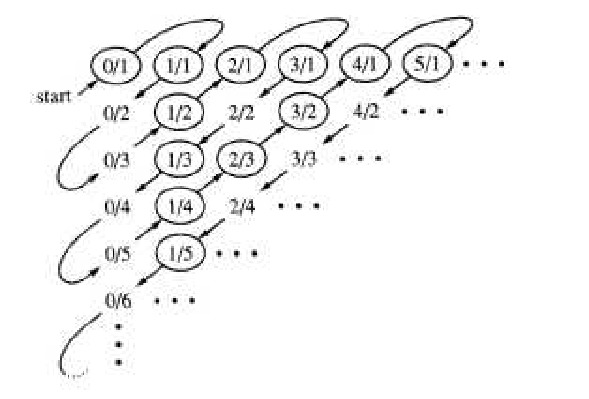
\includegraphics[width=1\linewidth]{images/fig-sol-7-2-9.png}
\caption{Enumeration of the rational numbers.
				 \label{fig-sol-7-2-9}}
\end{figure}
\item[10.]\hypertarget{exercise-18}{}\leavevmode%
\begin{enumerate}[label=\alph*]
\item\hypertarget{li-65}{} Prove that the set of finite strings of 0's and 1's is countable.%
\item\hypertarget{li-66}{}Prove that the set of odd integers is countable.%
\item\hypertarget{li-67}{}Prove that the set  \(\mathbb{N}\times  \mathbb{N}\) is countable.%
\end{enumerate}
%
\par\smallskip
\item[11.]\hypertarget{exercise-19}{} Use the Pigeonhole Principle to prove that an injection cannot exist between a finite set \(A\) and a finite set \(B\) if the
cardinality of \(A\) is greater than the cardinality of \(B\).%
\par\smallskip
\par\smallskip
\noindent\textbf{Answer.}\hypertarget{answer-9}{}\quad
 Let \(f\) be any function from \(A\) into \(B\). By the Pigeonhole principle with \(n=1\), there exists an element of \(B\) that is the image of at least two elements of \(A\). Therefore, \(f\) is not an injection.
%
\item[12.]\hypertarget{exercise-20}{} The important properties of relations are not generally of interest for functions. Most functions are not reflexive, symmetric, antisymmetric,
or transitive. Can you give examples of functions that do have these properties?%
\par\smallskip
\item[13.]\hypertarget{exercise-21}{} Prove that the set of all infinite sequences of 0's and 1's is not a countable set (i. e., that it is an uncountable set). %
\par\smallskip
\par\smallskip
\noindent\textbf{Answer.}\hypertarget{answer-10}{}\quad
 The proof is indirect and follows a technique called the Cantor diagonal process.
 Assume to the contrary that the set is countable, then the elements can be listed:

 \(n_1,n_2,n_3,\ldots\) where each \(n_i\) is an infinite sequence of 0s and 1s. Consider the array:
\[
\begin{array}{c}
n_1=n_{11}n_{12}n_{13}\cdots\\
n_2=n_{21}n_{22}n_{23}\cdots\\
n_3=n_{31}n_{32}n_{33}\cdots\\
\quad \vdots\\
\end{array}
\] 
%
\par
We assume that this array contains all infinite sequences of 0s and 1s. Consider the sequence \(s\) defined by

\(s_i=\begin{cases}
 0 & \textrm{ if } n_{\textrm{ii}}=1 \\
 1 & \textrm{ if } n_{\textrm{ii}}=0
\end{cases}\)
%
\par
Notice that \(s\) differs from each \(n_i\) in the \(i\)th position and so cannot be in the list. This is a contradiction, which completes our proof.%
\item[13.]\hypertarget{exercise-22}{} Prove that the set of all functions on the integers is an uncountable set.%
\par\smallskip
\end{exercisegroup}
\par\smallskip\noindent
\typeout{************************************************}
\typeout{Section 1.3 Function Composition}
\typeout{************************************************}
\section[Function Composition]{Function Composition}\label{s-function-composition}
\typeout{************************************************}
\typeout{Introduction  }
\typeout{************************************************}
Now that we have a good understanding of what a function is, our next step is to consider an important operation on functions. Our purpose is not
to develop the algebra of functions as completely as we did for the algebras of logic, matrices, and sets, but the reader should be aware of the
similarities between the algebra of functions and that of matrices. We first define equality of functions.%
\typeout{************************************************}
\typeout{Subsection 1.3.1 Function Equality}
\typeout{************************************************}
\subsection[Function Equality]{Function Equality}\label{ss-function-equality}
\begin{definition}[Equality of Functions]\label{def-equality-of-functions.}
\index{Function!Equality} Let \(f, g:A \rightarrow  B\); that is, let f and g both be functions from A into B.  Then f is
equal to g (i. e., \(f=g\)) if and only if \(f(x) = g(x)\) for all \(x \in  A\).%
\end{definition}
Two functions that have different domains cannot be equal. For example,  \(f: \mathbb{Z}\to \mathbb{Z}\) defined by \(f(x)=x^2\) and \(g: \mathbb{R}\to
\mathbb{R}\) defined by \(g(x)=x^2\) are not equal even though the formula that defines them is the same.%
\par
On the other hand, it is not uncommon for two functions to be equal even though they are defined differently. For example consider the functions
\(h\) and \( k\), where \(h: \{-1,0,1,2\}\to \{0,1,2\}\) is defined by \(h(x)=|x|\) and \(k: \{-1,0,1,2\}\to \{0,1,2\}\)
is defined by \(k(x) = -\frac{x^3}{3}+x^2+\frac{x}{3}\) appear to be very different functions. However, they are equal because \(h(x)= k(x)\)
for \(x = -1, 0, 1, \text{and} 2\).%
\typeout{************************************************}
\typeout{Subsection 1.3.2 Function Composition}
\typeout{************************************************}
\subsection[Function Composition]{Function Composition}\label{ss-composition}
One of the most important operations on functions is that of composition.%
\begin{definition}[Composition of Functions.]\label{def-composition-of-functions}
\index{Composition of Functions}\index{Function!Composition}\label{notation-5}
Let \(f:A \rightarrow  B\) and \(g:B \rightarrow  C\). Then the composition of f followed by g, written \(g\circ f\) is a function from A into C defined by \((g \circ f)(x) = g(f(x))\), which is read `` \(g\) of \(f\) of \(x\).''%
\end{definition}
\par
The reader should note that it is traditional to write the composition of functions from right to left. Thus, in the above definition, the first function performed in computing \(g \circ f\), which is \(f\). On the other hand, for relations, the composition \(r s\) is read from left
to right, so that the first relation is\(  r\).%
\begin{example}[A basic example]\label{ex-simple-composition}
Let \(f:\{1, 2, 3\}\rightarrow  \{a, b\}\) be defined by \(f(1) = a\), \(f(2) = a\), and \(f(3) = b\). Let \(g:\{a, b\} \rightarrow  \{5, 6, 7\}\) be defined by \(g(a) = 5\) and \(g(b) = 7\). Then \(g\circ f: \{1, 2, 3\}\rightarrow  \{5, 6, 7\}\) is defined by \((g\circ f)(1)= 5\),
\((g\circ f)(2)= 5,\) and \((g\circ f)(3)= 7\). For example, \((g\circ f)(1)= g(f(l)) = g(a) = 5\). Note that f\(circ\)g is not defined. Why?%
\par
 Let \(f:\mathbb{R} \rightarrow  \mathbb{R}\) be defined by \(f(x) = x^3\) and let \(g:\mathbb{R} \rightarrow  \mathbb{R}\) be defined by \(g(x)
= 3x+1\). Then, since

\quad \quad  \((g\circ f)(x) = g(f(x)) = g\left(x^3\right) = 3x^3 + 1\), 

we have \(g\circ f: \mathbb{R} \rightarrow  \mathbb{R}\) is defined by\((g\circ f)(x)= 3x^3 + 1\). Here \(f\circ g\) is also defined and \(f\circ
g:\mathbb{R}\rightarrow \mathbb{R}\) is defined by \((f\circ g)(x)=(3x + 1)^3\) . Moreover, since \(3x ^3+ 1 \neq (3x + 1)^3\) for at least
one real number, \(g\circ f \neq  f\circ g\).  Therefore, the commutative law is not true for functions under the operation of composition.
However, the associative law is true for functions under the operation of composition.
%
\end{example}
\begin{theorem}[Function composition is associative]\label{function-composition-associative}
If \(f:A\rightarrow B\),\(g:B\to C\), and \(h:C\rightarrow D\), then \(h\circ (g\circ f) = (h\circ g)\circ f\).%
\end{theorem}
\begin{proof}\hypertarget{proof-2}{}
Note: In order to prove that two functions are equal, we must use the definition of equality of functions. Assuming that the functions
have the same domain, they are equal if, for each domain element, the images of that element under the two functions are equal.%
\par
We wish to prove that \((h\circ (g\circ f))(x) = ((h\circ g)\circ f)(x)\) for all \(x \in  A\), which is the domain of both functions.%
\par

\((h\circ (g\circ f))(x)= h((g\circ f) (x))\textrm{   by the definition of composition}\\
\\
\quad \quad =h(g(f(x)))\textrm{   by the definition of composition}\)%
\par
Similarly,
\begin{equation*}((h\circ g)\circ f)(x)= (h\circ g)(f(x))\textrm{  by the definition of composition}\\
\\
\quad \quad =h(g(f(x)))\text{  }\textrm{  by the definition of composition}\end{equation*}%
\par
Notice that no matter how the functions the expression \(h\circ g\circ f\) is grouped, the final image of any element of \(x\in A\) is \(h(g(f(x)))\)
and so \(h\circ (g\circ f) = (h\circ g)\circ f\).  \(\square\)%
\end{proof}
\par
If \(f\) is a function from a set \(A\) onto itself, we can find \(f\circ  f\), \(f\circ  f\circ  f\), \(ldots\) ,which we write as
\(f^2\) , \(f^3\) , .... This idea can be expressed more elegantly as follows; If \(f: A \rightarrow  A\), the repeated composition of \textit{
f} with itself is defined recursively as;%
\begin{definition}[Powers of Functions]\label{def-powers-of-functions}
\index{Powers of Functions}\label{notation-6}
Let \(f: A\to A\).%
\par
\leavevmode%
\begin{itemize}[label=\textbullet]
\item{} \(f^1= f\);  that is, \(f^1(a) = f(a)\), for \(a \in A\).%
\item{} For \(n\geq 1\), \(f^{n+1}= f\circ f^n\);  that is, \(f^{n+1}(a)=f\left( f^n(a)\right)\) for \(a \in A\).%
\end{itemize}
%
\end{definition}
\par
Two useful theorems concerning composition are given below. The proofs are left for the exercises.%
\begin{theorem}[The composition of injections is an injection]\label{theorem-composition-of-injections}
If \(f: A \rightarrow  B\) and \(g : B \rightarrow  C\) are injections, then \(g\circ f : A \rightarrow  C\) is an injection.%
\end{theorem}
\begin{theorem}[title>The composition of surjections is a surjection]\label{theorem-composition-of-surjections}
 If \(f : A \rightarrow  B\) and \(g: B \rightarrow C\) are surjections, then \(g\circ f: A \rightarrow  C\) is a surjection.%
\end{theorem}
\par
We would now like to define the concepts of identity and inverse for functions under composition. The motivation and descriptions of the definitions
of these terms come from the definitions of the terms in the set of real numbers and for matrices. For real numbers, the numbers 0 and 1 play the
unique role that \(x + 0 = 0 + x = x\) and \(x \cdot 1 = 1 \cdot  x = x\) for any real number \(x\).  0 and 1 are the identity elements
for the reals under the operations of addition and multiplication, respectively. Similarly, the \(n \times  n\) zero matrix 0 and the \(n \times
 n\) identity matrix \(I\) are such that for any \(n \times  n\) matrix \(A\), \(A + 0 = 0 + A=A\) and \(A I = I A = I\). Hence, an
elegant way of defining the identity function under the operation of composition would be to imitate the above well-known facts.%
\begin{definition}[Identity Function]\label{def-identity-function}
\index{Identity Function}\label{notation-7}
For any set A, the identity function on A is a function from A onto A, denoted by i (or, more specifically, \(i_A\)) such that \(i(a) = a\)  for all \(a\in A\)%
\end{definition}
\par
Based on the definition of \(i\), we can show that for all functions \(f:A\to A\), \(f\circ i=i\circ f = f\).%
\begin{example}[The identity function on \(\{1,2,3\}\)]\label{ex-an-identity-function}
 If \(A = \{1, 2, 3\}\), then the identity function\(i : A \to  A\) is defined by \(i(1) = 1\), \(i(2) = 2,\) and \(i(3)= 3\).%
\end{example}
\begin{example}[The identity function on \(\mathbb{R}\)]\label{ex-identity-on-reals}
The identity function on \(\mathbb{R}\) is \(i : \mathbb{R} \rightarrow  \mathbb{R}\) defined by \(i(x) = x\).%
\end{example}
\typeout{************************************************}
\typeout{Subsection 1.3.3 Inverse Functions}
\typeout{************************************************}
\subsection[Inverse Functions]{Inverse Functions}\label{ss-inverse-functions}
We will introduce the inverse of a function with a special case: the inverse of a function on a set. After you've taken the time to understand this
concept, you can read about the inverse of a function from one set into another. The reader is encouraged to reread the definition of the inverse
of a matrix in Section 5.2 ({$\langle\langle$Unresolved xref, reference "def-matrix-inverse"; check spelling or use "provisional" attribute$\rangle\rangle$}) to see that the following definition of the inverse function is a direct analogue of that definition.%
\begin{definition}[ Inverse of a Function on a Set]\label{def-inverse-function}
\index{Inverse Function!of a function on a set}\label{notation-8}
 Let \(f: A\rightarrow  A\). If there exists a function \(g : A \rightarrow  A\) such that \(g\circ f = f\circ g = i\), then g is called the inverse of f and is denoted by \(f^{-1}\) , read ``f inverse.''%
\end{definition}
\par
Notice that in the definition we refer to ``the inverse'' as opposed to ``an inverse.''  It can be proven that a function can never have
more than one inverse (see exercises).%
\par
An alternate description of the inverse of a function, which can be proven from the definition, is as follows:  Let \(f: A \rightarrow  A\) be such that \(f(a) = b\). Then when it exists, \(f^{-1}\) is a function from \(A\) to \(A\) such that \(f^{-1}(b)=a\).
Note that \(f^{-1}\) ``undoes'' what \(f\) does. %
\begin{example}[The inverse of a function on \(\{1,2,3\}\)]\label{ex-simple-inverse}
Let \(A = \{1, 2, 3\}\) and let \(f\) be the function defined on \(A\) such that \(f(1) = 2\), \(f(2) = 3\), and
\(f(3) = 1\). Then \(f^{-1} : A \rightarrow  A\) is defined by \(f^{-1}(I) = 3\), \(f^{-1}(2) = 1\), and \(f^{-1}(3) = 2\).%
\end{example}
\begin{example}[Inverse of a real function]\label{ex-inverse-of-a-real-function}
If \(g : \mathbb{R} \rightarrow  \mathbb{R}\) is defined by \(g(x) =x^3\) , then \(g^{-1}\) is the function that undoes what
\(g\) does. Since \(g\) cubes real numbers, \(g^{-1}\) must be the ``reverse'' process, namely, takes cube roots. Therefore, \(g^{-1}
: \mathbb{R} \rightarrow  \mathbb{R}\) is defined by \(g^{-1}(x)=\sqrt[3]{x}\). We should show that \(g^{-1}\circ g = i\) and \(g\circ g^{-1}=i\).
We will do the first, and the reader is encouraged to do the second.

\(\left(g^{-1}\circ g\right)(x)= g^{-1}(g(x)) \quad \textrm{ Definition of composition}\\
\\
\text{       }= g^{-1}\left(x^3\right)\quad \text{Definition of } g\\
\\
\text{                       }=\sqrt[3]{x^3}\quad\textrm{Definition of } g^{-1}\\
\\
\text{                      }= x\quad\text{Definition of cube root}\\
\\
\text{     }= i(x)\quad\text{Definition of the identity function}\)%
\par
Therefore, \(g^{-1}\circ g = i\). Why?
%
\end{example}
\par
The definition of the inverse of a function alludes to the fact that not all functions have inverses. How do we determine when the inverse of a function
exists?%
\begin{theorem}[Bijections have inverses]\label{theorem-bijections-have-inverses}
Let \(f: A\rightarrow  A\).  \(f^{-1}\) exists if and only if f is a bijection; i. e. f is one-to-one and onto.%
\end{theorem}
\begin{proof}\hypertarget{proof-3}{}
(\(\Rightarrow\))  In this half of the proof, assume that \(f^{-1}\) exists and we must prove that \(f\) is one-to-one and onto.
To do so, it is convenient for us to use the relation notation, where \(f(s)=t\) is equivalent to \((s,t)\in f\). To prove that \(f\) is
one-to-one, assume that \(f(a)=f(b) = c\). Alternatively, that means \((a, c)\) and \((b, c)\) are elements of \(f\) . We must show
that \(a =b\). Since \((a, b), (c, b) \in \text{  }f\), \((c, a)\) and \((c,b)\) are in \(f^{-1}\) . By the fact that \(f^{-1}\) is a function
and \(c\) cannot have two images, \(a\) and \(b\) must be equal, so \(f\) is one-to-one. %
\par
Next, to prove that \(f\) is onto, observe that for \(f^{-1}\) to be a function, it must use all of its domain, namely A. Let \(b\)
be any element of \(A\). Then b has an image under \(f^{-1}\) , \(f^{-1}(b)\). Another way of writing this is \(\left(b,f^{-1}(b)\right)\in
f^{-1}\), By the definition of the inverse, this is equivalent to \(\left(f^{-1}(b), b\right) \in  f\). Hence, \(b\) is in the range of \(f\). Since \(b\) was chosen arbitrarily, this shows that the range of \( f \) must be all of \(A\).%
\par
(\(\Leftarrow\) ) Assume \(f\) is one-to-one and onto and we are to prove \(f^{-1}\) exists. We leave this half of the proof to the reader.
\(\square\)%
\end{proof}
\begin{definition}[Permutation]\label{def-Permutation}
\index{Permutation}A bijection of a set \(A\) into itself is called a permutation of \(A\).%
\end{definition}
\par
Next, we will consider the situation where \(f: A \rightarrow B\) and \(B\) is not necessarily equal to \(A\). How do we define the inverse in this case?%
\begin{definition}[Inverse of a Function (General Case) ]\label{def-general-inverse-function}
Let \(f:A \rightarrow  B\), If there exists a function \(g:B \rightarrow  A\) such that \(g \circ f = i_A\) and \(f\circ  g = i_B\) , then g is called the inverse of f and is denoted by \(f^{-1}\) , read ``f inverse.''%
\end{definition}
\par
Note the slightly more complicated condition for the inverse in this case because the domains of \(f\circ  g\) and \(g \circ f\) are different if
A and B are different. The proof of the following theorem isn't really very different from the special case where \(A=B\).%
\begin{theorem}[When does a function have an inverse?]\label{theorem-inverse-function-condition}
 Let\(f:A \rightarrow  B\). \(f^{-1}\) exists if and only if f is a bijection.%
\end{theorem}
\begin{example}[Another inverse]\label{example-inverse-another}
Let \(A =\{1,2, 3\}\) and \(B = \{a, b, c\}\). Define \(f:A \rightarrow  B\) by \(f(1) = a\), \(f(2) = b\), and {
}\(f(3) = c\). Then \(g: B \rightarrow  A\) defined by \(g(a) = 1\), \(g(b) = 2\), and \(g(c) = 3\) is the inverse of \(f\).

\[\left.
\begin{array}{c}
 (g\circ f)(1)= 1 \\
 (g\circ f)(2)=2 \\
 (g\circ f)(3)=3 \\
\end{array}
\right\}\Rightarrow \text{  }g\circ f = i_A \textrm{ and } \left.
\begin{array}{c}
 (f\circ g)(a)=a \\
 (f\circ g)(b)=b \\
 (f\circ g)(c)=c \\
\end{array}
\right\}\Rightarrow \text{  }f\circ g = i_B\]%
\end{example}
\typeout{************************************************}
\typeout{Exercises 1.3.4 Exercises for Section 7.3 }
\typeout{************************************************}
\subsection[Exercises for Section 7.3 ]{Exercises for Section 7.3 }\label{exercises-7-3}
\hypertarget{exercisegroup-5}{}\typeout{************************************************}
\typeout{Introduction  }
\typeout{************************************************}
A Exercises%
\begin{exercisegroup}
\item[1.]\hypertarget{exercise-23}{}Let \(A = \{1,2, 3, 4, 5\}\), \(B = \{a, b, c, d, e,f\}\), and \(C = \{+, -\}\). Define \(f: A \to  B\) by \(f(k)\) equal to the \(k^{th}\)
letter in the alphabet, and define \(g : B \rightarrow  C\) by \(g(\alpha ) = +\) \textrm{ if }\(alpha\) is a vowel and \(g(\alpha ) = -\) \textrm{ if } \textit{
\(alpha\)} is a consonant.%
\par
\leavevmode%
\begin{enumerate}[label=\alph*]
\item\hypertarget{li-70}{} Find \(g\circ  f\).%
\item\hypertarget{li-71}{} Does it make sense to discuss \(f\circ g\)? If not, why not?%
\item\hypertarget{li-72}{} Does \(f^{-1}\) exist? Why?%
\item\hypertarget{li-73}{} Does \(g^{-1}\) exist? Why?%
\end{enumerate}
%
\par\smallskip
\par\smallskip
\noindent\textbf{Answer.}\hypertarget{answer-11}{}\quad
\leavevmode%
\begin{enumerate}[label=\alph*]
\item\hypertarget{li-74}{}  \(g\circ f:A\to C\) is defined by \((g\circ f)(k)=\begin{cases}
 + & \text{if} k=1 \text{or} k=5 \\
 - & \text{if} k=2,3,4
\end{cases}\)%
\item\hypertarget{li-75}{} No, since the domain of \(f\) is not equal to the codomain of \(g\).%
\item\hypertarget{li-76}{} No, since \(f\) is not surjective.%
\item\hypertarget{li-77}{} No, since \(g\) is not injective.%
\end{enumerate}
%
\item[2.]\hypertarget{exercise-24}{} Let \(A = \{1, 2, 3\}\). Define\(f:A\rightarrow A\) by \(f(1) = 2\), \(f(2) = 1\), and \(f(3) = 3\). Find \(f^2\) , \(f^3\) , \(f^4\) and
\(f^{-1}\).%
\par\smallskip
\item[3.]\hypertarget{exercise-25}{}Let \(A = \{1, 2, 3\}\).%
\par
\leavevmode%
\begin{enumerate}[label=\alph*]
\item\hypertarget{li-78}{} List all permutations of \(A\).%
\item\hypertarget{li-79}{} Find the inverse of each of the permutations of part a.%
\item\hypertarget{li-80}{} Find the square of each of the permutations of part a.%
\item\hypertarget{li-81}{} Show that the composition of any two permutations of \(A\) is a permutation of \( A\).%
\item\hypertarget{li-82}{} Prove that if \(A\) be any set where the \(|A|=\text{\textit{$n$}}\), then the number of permutations of \(A\) is \(n!\).%
\end{enumerate}
%
\par\smallskip
\par\smallskip
\noindent\textbf{Answer.}\hypertarget{answer-12}{}\quad
\leavevmode%
\begin{enumerate}[label=\alph*]
\item\hypertarget{li-83}{} The permutations of \(A\) are \(i,r_1,r_2,f_1,f_2,\) and \(f_3\), defined in section 15.3
%
\item\hypertarget{li-84}{}    
 \[\begin{array}{ccc}
g  & g^{-1} & g^2 \\
 i & i & i \\
r_1 & r_2 & r_2 & \\
r_2 & r_1 & r_1 & \\
f_1 & f_1 & i & \\
f_2 & f_2 & i & \\
f_3 & f_3 & i & \\
\end{array}\]%
\item\hypertarget{li-85}{} Apply both Theorems 7.3.3 and 7.3.4: If \(f\) and \(g\) are permutations of \(A\), then they are both  \\
 injections and their composition, \(f\circ g\), is a injection, by Theorem 7.3.3. By 7.3.4, \(f\circ g\) is also a \\
 surjection; therefore, \(f\circ g\) is a bijection on \(A\), a permutation.%
\item\hypertarget{li-86}{} Proof by induction: Basis: \((n=1)\).  The number of permutations of \(A\) is one, the identity function, and 1! \(=1\).%
\par
Induction: Assume that the number of permutations on a set with \(n\) elements,
 \(n\geq 1\), is \(n\)!. Furthermore, assume that \(|A|=\)\(\text{  }n+1\) and that \(A\) contains
  an element called \(x\). Let \(A'=A-\{x\}\). We can reduce the definition of a permutation, \(f\),
   on \(A\) to two steps. First, we select any one of the \(n\)! permutations on \(A'\).
    (Note the use of the induction hypothesis.) Call it \(g\). This permutation almost
     completely defines a permutation on \(A\) by \(f\) for all
      \(a\) in \(A'\), Next, we select the image of \(x\), which can be done \(n+1\) different ways.
       To keep our function bijective, we must adjust \(f\) as follows: If we select \(f(x)=y\),
        then we must find the element, \(z\), of \(A\) such that \(g(z)=y\), and redefine the image
         of \(z\) to \(f(z)=x\). If we had selected \(f(x)=x\), then there is really no adjustment needed.
          By the rule of products, the number of ways that we can define \(f\) is \(n!(n+1)=(n+1)!\) \(\square\)%
\end{enumerate}
%
\item[4.]\hypertarget{exercise-26}{} Define \(s\), \(u\), and \(d\), all functions on the integers, by \(s(n) = n^2\) , \(u(n) = n + 1\), and \(d(n) = n-1\). Determine:%
\par
\leavevmode%
\begin{enumerate}[label=\alph*]
\item\hypertarget{li-87}{} \(u \circ  s \circ  d\)%
\item\hypertarget{li-88}{} \(s \circ  u\circ  d\)%
\item\hypertarget{li-89}{} \(d \circ  s \circ  u\)%
\end{enumerate}
%
\par\smallskip
\item[5.]\hypertarget{exercise-27}{} Based on the definition of the identity function, show that for all functions \(f:A\to A\), \(f\circ i=i\circ f = f\).%
\par\smallskip
\item[6.]\hypertarget{exercise-28}{}\terminology{Inverse images.} If \(f\) is any function from \(A\) into \(B\), we can describe the inverse image of from \textit{
B }into \(\mathcal{P}(A)\), which is also commonly denoted \(f^{-1}\). If \(b \in  B\), \(\left.f^{-1}(b) = \{a \in A | f(a) = b\right)\). If
\(f\) does have an inverse, the inverse image of \(b\) is \(\left\{f^{-1}(b)\right\}\).%
\par
\leavevmode%
\begin{enumerate}[label=\alph*]
\item\hypertarget{li-90}{} Let \(g : \mathbb{R} \to  \mathbb{R}\) be defined by \(g(x) = x^2\). What are \(g^{-1}(4)\), \(g^{-1}(0)\) and \(g^{-1}(-1)\)?%
\item\hypertarget{li-91}{} If \(r: \mathbb{R}\to \mathbb{Z}\), where \(r(x) = \lceil x\rceil\),  what is \(r^{-1}(1)\)?%
\end{enumerate}
%
\par\smallskip
\item[7.]\hypertarget{exercise-29}{} Let \( f,\)  \(g\), and \(h\) all be functions from \(\mathbb{Z}\) into \(\mathbb{Z}\) defined by \(f(n) = n + 5\), \(g(n) = n - 2,\)
and \(h(n)=n^2\). Define:%
\par
\leavevmode%
\begin{enumerate}[label=\alph*]
\item\hypertarget{li-92}{} \(f\circ g\)%
\item\hypertarget{li-93}{} \(f^3\)%
\item\hypertarget{li-94}{} \(f\circ h\)%
\end{enumerate}
%
\par\smallskip
\par\smallskip
\noindent\textbf{Answer.}\hypertarget{answer-13}{}\quad
\leavevmode%
\begin{multicols}{3}
\begin{enumerate}[label=\alph*]
\item\hypertarget{li-95}{} \(f\circ g(n)=n+3\)%
\item\hypertarget{li-96}{} \(f^3(n)=n+15\)   %
\item\hypertarget{li-97}{} \(f\circ h(n)=n^2+5\) %
\end{enumerate}
\end{multicols}
%
\item[8.]\hypertarget{exercise-30}{}Define the following functions on the integers by \(f(k) = k + 1\), \(g(k) = 2k\), and \(h(k)=\lceil k/2\rceil\) %
\par
\leavevmode%
\begin{enumerate}[label=\alph*]
\item\hypertarget{li-98}{} Which of these functions are one-to-one?%
\item\hypertarget{li-99}{} Which of these functions are onto?%
\item\hypertarget{li-100}{} Express in simplest terms the compositions \(f\circ g\), \(g \circ f\), \(g \circ  h\), \(h \circ  g\), and \(h^2\) ,%
\end{enumerate}
%
\par\smallskip
\item[9.]\hypertarget{exercise-31}{} Let \(A\) be a nonempty set. Prove that if \( f \) is a bijection on \(A\) and \(f\circ f=f\), then \( f \)is the identity
function, \(i\) %
\par\smallskip
\par\smallskip
\noindent\textbf{Hint.}\hypertarget{hint-1}{}\quad
You have seen a similar proof in matrix algebra.%
\item[10.]\hypertarget{exercise-32}{} For the real matrix \(A=\left(
\begin{array}{cc}
 a & b \\
 c & d \\
\end{array}
\right), \text{\textit{\det }} A=\text{\textit{ad}-\text{bc}}\).%
\par
Recall that a  \terminology{bijection} from a set to itself is also referred to as a \terminology{permutation} of the set. Let \(\pi\) be a permutation of \(\{a,b,c,d\}\) such that \(a\) becomes \(\pi (a)\), \(b\) becomes \(\pi (b)\), etc.%
\par
Let \(B=\left(
\begin{array}{cc}
 \pi(a)& \pi(b)\\
 \pi(c)& \pi(d)\\
\end{array}
\right)\). How many permutations of \(pi\) leave the determinant of \(A\) invariant, that is, \(\det  A = \det  B\)?%
\par\smallskip
\end{exercisegroup}
\par\smallskip\noindent
\hypertarget{exercisegroup-6}{}\typeout{************************************************}
\typeout{Introduction  }
\typeout{************************************************}
B Exercises%
\begin{exercisegroup}
\item[11.]\hypertarget{exercise-33}{}State and prove a theorem on inverse functions analogous to the one that says that f a matrix hais an inverse, that inverse is unique.%
\par\smallskip
\par\smallskip
\noindent\textbf{Answer.}\hypertarget{answer-14}{}\quad
If \(f:A\to B\) and \(f\) has an inverse, then that inverse is unique.%
\par
Proof:  Suppose that \(g\) and \(h\) are both inverses of \(f\).

\[
\begin{split}g &= g\circ i_A \\
		& =g\circ (f\circ h)\\
		& =(g\circ f)\circ h\\
		& =i_A\circ h\\
		& = =h\quad \Rightarrow g=h \quad \square
\end{split}
\]
		%
\item[12.]\hypertarget{exercise-34}{} Let \(f\) and \(g\) be functions whose inverses exist. Prove that \((f\circ g)^{-1}= g^{-1}\circ f^{-1}\).%
\par\smallskip
\par\smallskip
\noindent\textbf{Hint.}\hypertarget{hint-2}{}\quad
See Exercise 3 of Section 5.4.%
\item[13.]\hypertarget{exercise-35}{} Prove \hyperref[theorem-composition-of-injections]{Theorem~\ref{theorem-composition-of-injections}} and \hyperref[theorem-composition-of-surjections]{Theorem~\ref{theorem-composition-of-surjections}}.%
\par\smallskip
\par\smallskip
\noindent\textbf{Answer.}\hypertarget{answer-15}{}\quad
 Let \(x,x'\) be elements of \(A\) such that \(g\circ f(x)=g\circ f(x')\); that is, \(g(f(x))=g(f(x'))\). Since \(g\) is injective, \(f(x)=f(x')\) and since \(f\) is injective, \(x=x'\). \(\square\)%
\par
 Let \(x\) be an element of \(C\). We must show that there exists an element of \(A\) whose image under \(g\circ f\) is \(x\). Since \(g\) is surjective, there exists an element of \(B\), \(y\), such that \(g(y)=x\). Also, since \(f\) is a surjection, there exists an element of \(A\), \(z\), such that \(f(z)=y\), \(g\circ f(z)=g(f(z))=g(y)=x\).\(\square\)%
\item[14.]\hypertarget{exercise-36}{} Prove the second half of \hyperref[theorem-bijections-have-inverses]{Theorem~\ref{theorem-bijections-have-inverses}}.%
\par\smallskip
\item[15.]\hypertarget{exercise-37}{} Prove by induction that if \(n\geq  2\) and \(f_1\), \(f_2\) , \ldots  , \(f_n\) are invertible functions on some nonempty set A, then {
}\(\left( f_1\circ  f_2\circ  \cdots  \circ  f_n \right){}^{-1}= f_n^{-1}\circ \cdots \circ f_2^{-1}\circ f_1^{-1}\). The basis has been taken
care of in Exercise 10.%
\par\smallskip
\par\smallskip
\noindent\textbf{Answer.}\hypertarget{answer-16}{}\quad
Basis: \((n=2)\): \(\left(f_1\circ f_2\right){}^{-1}=f_2{}^{-1}\circ f_1{}^{-2}\) by exercise 10. %
\par
Induction: Assume \(n\geq 2\) and \(\left(f_1\circ f_2\circ \cdots \circ f_n\right){}^{-1}=\)\\
 \(f_n{}^{-1}\circ \cdots \circ f_2{}^{-1}\circ f_1{}^{-1}\)\\
 Consider \(\left(f_1\circ f_2\circ \cdots \circ f_{n+1}\right){}^{-1}\).
  \(\left(f_1\circ f_2\circ \cdots \circ f_{n+1}\right){}^{-1}\) \(=\left(\left(f_1\circ f_2\circ \cdots \circ f_n\right)\circ f_{n+1}\right){}^{-1}\)\\
  by the Basis   \(=f_{n+1}{}^{-1}\circ \left(f_1\circ f_2\circ \cdots \circ f_n\right){}^{-1}\)\\
  by Induction hypothesis  \(=f_{n+1}{}^{-1}\circ \left(f_n{}^{-1}\circ \cdots \circ f_2{}^{-1}\circ f_1{}^{-1}\right)\)\\
 \(=f_{n+1}{}^{-1}\circ \cdots \circ f_2{}^{-1}\circ f_1{}^{-1}\). \(\square\)
 %
\end{exercisegroup}
\par\smallskip\noindent
\hypertarget{exercisegroup-7}{}\typeout{************************************************}
\typeout{Introduction  }
\typeout{************************************************}
C Exercises%
\begin{exercisegroup}
\item[16.]\hypertarget{exercise-38}{}\leavevmode%
\begin{enumerate}[label=\alph*]
\item\hypertarget{li-101}{} Our definition of cardinality states that two sets, \(A\) and \(B\), have the same cardinality if there exists a bijection
between the two sets. Why does it not matter whether the bijection is from \(A\) into \(B\) or \(B\) into \(A\)?%
\item\hypertarget{li-102}{}Prove that ``has the same cardinality as'' is an equivalence relation on sets.%
\end{enumerate}
%
\par\smallskip
\item[17.]\hypertarget{exercise-39}{}Construct a table listing as many ``Laws of Function Composition'' as you can identify. Use previous lists of laws as a guide.%
\par\smallskip
\end{exercisegroup}
\par\smallskip\noindent
%
\backmatter
%
%
%% A lineskip in table of contents as transition to appendices, backmatter
\addtocontents{toc}{\vspace{\normalbaselineskip}}
%
\typeout{************************************************}
\typeout{References  References}
\typeout{************************************************}
\chapter[References]{References}\label{references-1}
%% If this is a top-level references
%%   you can replace with "thebibliography" environment
\begin{referencelist}
\bibitem[1]{biblio-sopowit-1983}\hypertarget{biblio-sopowit-1983}{}Sopowit, K. J., E. M. Reingold, and D. A. Plaisted \textit{The Traveling Salesman Problem and Minimum Matching in the Unit Square}.SIAM J. Computing, 1983,\textbf{12}, 144\textendash{}56.
\end{referencelist}
%
%% The index is here, setup is all in preamble
\printindex
%
\end{document}